% Metodología e implementación

\chapter*{Implementación} \label{cap5}
\addcontentsline{toc}{chapter}{Implementación}

\begin{flushright}
\begin{minipage}{7.85cm}
    {\em Si necesitas más de tres niveles de indentación estás jodido, y
    deberías arreglar tu programa.} \\  Linus Torvalds
\end{minipage}
\end{flushright}

\vspace*{5mm}

\section*{Metodología}

Al ser este un proyecto de tamaño considerable, y al realizarse en grupo, es
necesario establecer una metodología para evitar el trabajo inútil o redundante.

Para organizar nuestro trabajo, y poder mantener siempre cierto control sobre la
evolución de la aplicación, nos hemos servido tanto de herramientas como de
algunas buenas prácticas.

Habiendo desarrollado nuestro proyecto en el marco del IV CUSL\footnote{Concurso
Universitario de Software Libre: \url{http://www.concursosoftwarelibre.org}}
hemos seguido una política de divulgación de la información y unos plazos de
entrega. Desde la organización del concurso pusieron a nuestra disposición una
forja, en concreto la forja
IRIS-Libre\footnote{\url{https://forja.rediris.es/projects/cusl4-catastrof/}},
gracias a la que pudimos agilizar y centralizar las labores de administración y
planificación del proyecto.

Además adoptamos una política de entrevistas frecuentes con los tutores para
así motivarnos y que nos aconsejaran sobre el mejor paso a seguir, o en dónde
deberíamos profundizar más, o cuándo seguir otras vías de investigación.

De esta manera teníamos objetivos a corto plazo, herramientas para la
planificación gracias al IV CUSL, y guía por parte de los tutores.

\subsection*{Metodologías Ágiles}

Una buena planificación no implica el éxito, pero por lo menos te asegura unos
resultados mínimos.

No hemos aplicado ninguna metodología en concreto, si no un conjunto de técnicas
y buenos métodos. Creemos en una metodología de desarrollo ágil.

\subsubsection*{Reuniones de Desarrollo}

Lo principal es la comunicación entre los desarrolladores, para ello decidimos
reunirnos y comentar las avances o principales problemas al menos dos veces a
la semana.

Las reuniones no tenían por qué ser en persona, ni muy formales, podían
realizarse a través de mensajería instantánea, ayudados con herramientas de
pizarras virtuales. De esta forma siempre se tiene una idea muy cercana del
desarrollo del proyecto sin perder mucho tiempo.

Además mantiene un fuerte lazo entre los desarrolladores y les permite ayudarse
unos a otros, evitando así estancamientos o frustraciones con problemas
difíciles.

\subsubsection*{Reuniones con los Tutores}

Nos reuníamos con nuestros tutores al menos dos veces al mes, dependiendo del
ritmo de trabajo y progresos. Estas reuniones eran de carácter informativo y
orientativo.

Las reuniones permiten un crecimiento guiado y controlado del producto final, y
un nivel de acabado mayor al centrarnos solo en las partes realmente importantes
de la investigación y el desarrollo para los objetivos del proyecto.

\subsubsection*{Sistema Incremental}

Lo principal era desarrollar una plataforma muy básica y sencilla donde se
pudieran llevar a cabo pruebas, y una vez completada, ir aumentando las
prestaciones en forma de módulos o complementos que fueran implementando las
funcionalidades deseadas.

Seguimos pues un modelo iterativo de desarrollo del software, que es el ciclo
de vida del software que probablemente mejor se adapte a metodologías ágiles.

% TODO esquema del ciclo de vida iterativo

\subsubsection*{Reparto de Tareas Dinámico}

El reparto de tareas equitativo y ágil es vital para mantener una buena
relación entre los desarrolladores, y para el adecuado progreso del proyecto.

Por ello es importante identificar las tareas a realizar e ir asignándolas a
los desarrolladores, de forma que ellos mismos puedan decidir cómo organizarse,
pero siempre teniendo en cuenta unos plazos finales.

El reparto no siempre es estático, puesto que las tareas se pueden alargar o
acortar debido a una mala estimación inicial, incluso a veces se pueden
reasignar o subdividir para agilizar el desarrollo.

Al haber más de un desarrollador en el proyecto hemos tendido un poco a la
especialización en las tareas. Si un desarrollador ha estado trabajando en una
parte, o tiene experiencia y aptitudes para determinado aspecto del desarrollo,
tendrá prioridad a la hora de asignar las tareas relacionadas.

Sin embargo, no se trata de dividir el proyecto en dos, puesto que siempre se
intenta que todos los desarrolladores estén implicados en todas las ramas.
Después de todo el objetivo final del proyecto es aprender y ampliar
conocimientos en todas las áreas que éste toca.

\subsection*{Forja IRIS-Libre}

RedIRIS proporciona un servicio de forja bajo el nombre de
IRIS-Libre\footnote{\url{https://forja.rediris.es/}}. Esta forja proporciona
alojamiento y herramientas a proyectos de Software Libre, y está asociada al
CUSL, dando alojamiento a los proyectos participantes.

\begin{figure}[H]
 \centering
 
\includegraphics[width=30mm]{figuras/cap5/iris_libre.png}
 \caption{Logo de IRIS-Libre}
\end{figure}

Entre las herramientas para el alojamiento y la gestión de proyectos de carácter
colaborativo, y con vistas de crear una comunidad de desarrolladores, que
proporciona encontramos:

\subsubsection*{Subversion}

Como sistema de control de versiones la forja proporciona
SVN\footnote{\url{http://subversion.tigris.org/}}, este sistema permite llevar
un control sobre los cambios en el código, y obtener siempre una copia
actualizada con la última versión.

\begin{figure}[H]
 \centering
 
\includegraphics[width=80mm]{figuras/cap5/svn.png}
 \caption{Logo de Subversion}
\end{figure}

Este tipo de software es imprescindible cuando se trabaja en grupo, pues
facilita la colaboración y permite mantener un orden en el desarrollo.

\subsubsection*{Planificador de Tareas}

La forja también dispone de una sencilla aplicación de control de tareas, que,
entre otras cosas, lo que permite es:

\begin{enumerate}
 \item Crear una tarea, con una breve descripción de la misma.
 \item Asignarlas a un desarrollador, y así poder repartir la carga de trabajo.
 \item Estimación del tiempo necesario, para poder planificar otras tareas.
 \item Progreso de la tarea, para poder hacer un seguimiento del progreso de la
 misma.
 \item Fecha límite de finalización.
\end{enumerate}

Con estos sencillos parámetros la herramienta incluso genera un diagrama de
Gantt para ayudarte con la planificación.

% TODO incluir dicho diagrama

\subsection*{Blog}

La decisión de comenzar un blog para registrar la evolución del proyecto viene
motivada por el CUSL, que lo exige como requisito de los proyectos
participantes.

El llevar al día un blog\footnote{Simulación de Catástrofes:
\url{http://pfc.mensab.com/}}, con las actualizaciones y las direcciones
generales de desarrollo del proyecto, es algo altamente recomendable si se
quiere que el proyecto cree una comunidad. Es una manera muy cómoda y eficaz de
mantener a la comunidad informada de los cambios y el estado del proyecto.

Además también tiene otras consecuencias más sutiles; por ejemplo, permite
reafirmar las decisiones de diseño o de desarrollo tomadas a lo largo de la
implementación, puesto que queda constancia de las decisiones tomadas y las
razones para llevarlas a cabo.

\subsection*{Git}

Git\footnote{Git - Fast Version Control System: \url{http://git-scm.com/}} es
un sistema de control de versiones distribuido con filosofía distinta a la de
SVN, que es centralizado.

\begin{figure}[H]
 \centering
 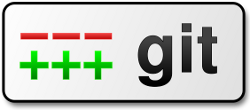
\includegraphics[width=40mm]{figuras/cap5/git.png}
 \caption{Logo de Git}
\end{figure}

En cada proyecto colaborativo hay muchos desarrolladores que necesitan hacer
muchos cambios, probar muchas alternativas de su código y sin embargo mantener
a todo el mundo informado y a su vez mantener una rama estable de desarrollo.
SVN no es demasiado eficiente a la hora de gestionar diferentes ramas de
desarrollo, ni al crearlas ni al unirlas.

Git soluciona este problema al fomentar los {\em commits} pequeños y una
herramienta de {\em merge} más eficiente, lo que facilita trabajar con ramas y
mantenerlas muy fácilmente. El trabajo con diferentes ramas de desarrollo y
una rama {\em master} siempre funcional, de fácil integración entre sí, facilita
el desarrollo considerablemente. Git fomenta este estilo de desarrollo.

Con su sistema de log y sus normas de estilo mejora el seguimiento de todos los
cambios, muy bien documentados, del código.

Por estas razones decidimos migrar la aplicación de SVN a Git cuando terminó el
CUSL. Esta migración nos obligó a buscar una nueva forja que nos proporcionara
este avanzado sistema de control de versiones. La elegida fue
Gitorious\footnote{\url{http://gitorious.org/}}, forja libre para proyectos
libres.

\begin{figure}[H]
 \centering
 
\includegraphics[width=40mm]{figuras/cap5/gitorious.png}
 \caption{Logo de Gitorious}
\end{figure}

\section*{Escenario de Simulación}

El escenario de simulación es la manera que tenemos de decirle a nuestro
simulador qué es lo que queremos simular precisamente. Dado que el simulador es
versátil y tiene capacidad de simular, en principio, cualquier lugar, hay que
definir una serie de parámetros de entrada.

En un escenario hemos de especificar cuál es el área con la que se va a
trabajar, cuáles son las entradas de agua y qué agentes humanos intervienen.
Aparte se definen también algunos parámetros técnicos como pueden ser los datos
de conexión a la base de datos de alturas.

Entrando en detalles los elementos de los que consta un escenario son:

\begin{description}
 \item[Nombre y descripción] Los escenarios se nombran para poder
identificarlos con facilidad, este nombre y descripción se muestra también en
los resultados de la simulación.
 \item[Fecha y hora] También se define la fecha y hora del comienzo de la
simulación, lo que permite localizar en el tiempo cada momento de la simulación.
 \item[Resolución temporal] Es necesario definir el tiempo transcurrido entre
dos estados de la simulación, tanto el tiempo simulado (en minutos) que
transcurre, como el tiempo de ejecución (en milisegundos) que se le concede a
la máquina -o máquinas- para simular un paso.
 \item[Área de simulación] El área viene definida por dos coordenadas
geográficas, la coordenada noroeste y la sureste del rectángulo -en realidad
no es un rectángulo si tenemos en cuenta la curvatura terrestre- que definen si
tomamos como diagonal el segmento que las une.
 \item[Resolución espacial] Uno de los parámetros más importantes que hay que
definir es la resolución espacial, tanto superficial como en altura. Hay que
especificar el tamaño de los hexágonos, lo que se hace a través del diámetro de
la circunferencia circunscrita en ellos -los hexágonos son regulares-. También
hay que definir la resolución espacial en altura, es decir, cómo se discretiza
la altura del terreno y del agua; se define como \begin{math}^1/_p\end{math}
metros de precisión donde {\em p} es el parámetro que aparece en el escenario.
 \item[Agentes Entorno] El número de agentes Entorno que se encargaran de
simular el escenario, el número adecuado depende de la cantidad de núcleos o
procesadores del que disponga la máquina donde se lleve a cabo la simulación.
 \item[Base de datos de alturas] En el escenario se incluyen también los datos
necesarios para realizar la conexión a la base de datos donde se almacenan la
elevación del terreno. Estos datos se obtienen de internet, pero se almacenan
localmente para agilizar simulaciones sucesivas en el mismo área.
 \item[Entradas de agua] A la hora de simular una inundación es básico simular
dónde y cuánta agua está entrando al sistema. Dichos datos se encuentran en el
escenario.
 \item[Peatones] La posición y características de los peatones, tales como su
distancia de visión, velocidad y objetivos -refugios que conocen de antemano-.
 \item[Frecuencia de actualización de resultados] Cada cuánto tiempo deben los
agentes Entorno enviar el estado de la simulación a los agentes encargados de
mostrar los resultados, así se define la finura de los resultados obtenidos.
\end{description}

Hay que destacar que los datos definidos en el escenario son los datos
iniciales de la simulación, y que muchos se traducen a agentes, como por
ejemplos las entradas de agua o las personas. Esto permite que en caliente se
puedan añadir, por ejemplo, nuevas fuentes de agua a la simulación, pues se
puede añadir agentes nuevos a una simulación en marcha.

\subsection*{Ejemplo de Escenario}

\lstinputlisting[caption=Escenario de ejemplo]{capitulo5/Ejemplo.scen}

Como se puede ver en el listado el formato de los ficheros escenario es {\em
clave=valor}, y para escribir un array -que son anidables, como se puede ver
también en el ejemplo- {\em clave=[elem,elem,elem...]}.

Lo primero que aparece es el {\em type}, es decir, el tipo de escenario del que
se trata. El valor es el nombre de la clase que hay que instanciar -que debe
heredar de {\em util.Scenario}-, por ahora sólo está implementado el caso de la
inundación, pero el escenario está preparado para múltiples tipos de desastres.

Es importante destacar que el orden en el que aparecen los elementos del
escenario en el fichero es irrelevante, cualquier orden es válido siempre que
aparezcan los elementos mínimos.

A continuación en el ejemplo aparecen el nombre ({\em name}), descripción ({\em
description}), fecha de inicio de la simulación ({\em date}) y hora inicial
({\em hour}).

Los dos siguientes elementos, {\em tick} y {\em realTick}, representan el
tiempo asignado a cada paso de la simulación. El primero se mide en
milisegundos y representa el tiempo de computación, es el que transcurre en
nuestro mundo; y el segundo se mide en minutos y representa cuanto tiempo ha
pasado dentro de la simulación.

{\em NW} y {\em SE} son dos arrays con las coordenadas geográficas de las dos
esquinas del área de simulación. Al igual que el resto de coordenadas que
aparecen en el escenario se escriben con el formato {\em [latitud,longitud]}.
{\em NW} hace referencia a la esquina noroeste, mientras que {\em SE}
referencia a la sureste.

{\em tileSize} corresponde al tamaño de los hexágonos, en metros, mientras que
{\em precision} define la resolución espacial en altura, en
\begin{math}^1/_{precision}\end{math} metros.

Seguido aparece el número de agentes {\bf Entorno}, con la clave {\em numEnvs}.
{\em randomTerrain} es un valor booleano que define si los entornos van a
utilizar datos reales de alturas, o van a generar terrenos aleatorios. Los dos
posibles valores que puede tomar son {\em True} y {\em False}, significando el
primero que el terreno simulado va a ser aleatorio.

A continuación vienen los datos necesarios para la conexión con la base de
datos de alturas. Todos comienzan por {\em DB}. {\em DBServer} es la url, ip,
nombre de fichero, etc, del servidor de base de datos. En este caso se trata de
un servidor que se encuentra en la misma máquina, y al que se accede por red
-de ahí las {\em //}-. {\em DBPort} es el puerto a usar para la conexión. {\em
DBUser} es el usuario con el que identificarse, y {\em DBPass} es la contraseña
en claro a utilizar. {\em DBDriver} especifica qué tipo de servidor se está
utilizando, en este caso se utiliza MySQL\footnote{\url{http://www.mysql.com/}}.
{\em DBDb} es el nombre de la base de datos donde se encuentra la tabla
{\bf Elevations}, dicha tabla está descrita en la sección donde se trata la
obtención de datos de alturas.

No todos los elementos {\em DB} son imprescindibles. Por ejemplo, si se utiliza
el servidor de base de datos de fichero
SQLite\footnote{\url{http://www.sqlite.org/}} no es necesario definir más que
{\em DBServer} y {\em DBDriver}.

Cada línea con la clave {\em waterSource} representa una entrada de agua
diferente al sistema, todas las entradas definidas en el fichero del escenario
se activan nada más comenzar la simulación. Para añadir fuentes de agua que
aparecen un tiempo después del comienzo de la simulación hay que añadir agentes
{\bf Entrada de Agua} en caliente. El array contiene los siguientes datos:
latitud, longitud y cantidad de agua que entra en cada tick medida en unidades
de altura de la simulación. El orden en que aparecen estos elementos es fijo.

Al igual que con las entradas de agua, puede haber múltiples líneas con la clave
{\em person}. Representan a agentes {\bf Peatón} en la simulación. Los
parámetros del array son, en orden, los siguientes: latitud, longitud,
distancia de visión en hexágonos, velocidad en hexágonos, número de clones y un
array de objetivos -con múltiples pares latitud y longitud, aunque en este caso
sólo hay un objetivo-. Todos estos parámetros serán discutidos en la sección de
los agentes {\bf Peatón}.

{\em updateTimeKML} y {\em updateTimeVisor} se miden ambos en milisegundos, y
hacen referencia al tiempo que transcurre entre que los agentes {\bf Entorno}
envían actualizaciones a los generadores de KML y a los visores respectivamente.

\subsection*{Generación de Escenarios}

Aunque es perfectamente posible escribir un fichero escenario con un editor de
textos, resulta más sencillo utilizar el script de lanzamiento de la simulación
para generar uno en un modo interactivo. Dicho modo se explica en detalle en la
sección dedicada al script de lanzamiento.

\section*{Agentes}

En esta sección se explicarán uno a uno todos los agentes que intervienen en la
simulación, y cómo se han implementado. Todos los agentes se encuentran en el
paquete, o en subpaquetes de éste, {\em agents}.

A continuación sigue un esquema con todos los agentes del simulador, los
comportamientos que utiliza cada agente, y flechas entre agentes que denotan
qué agentes se comunican entre sí.

\begin{figure}[H]
 \centering
 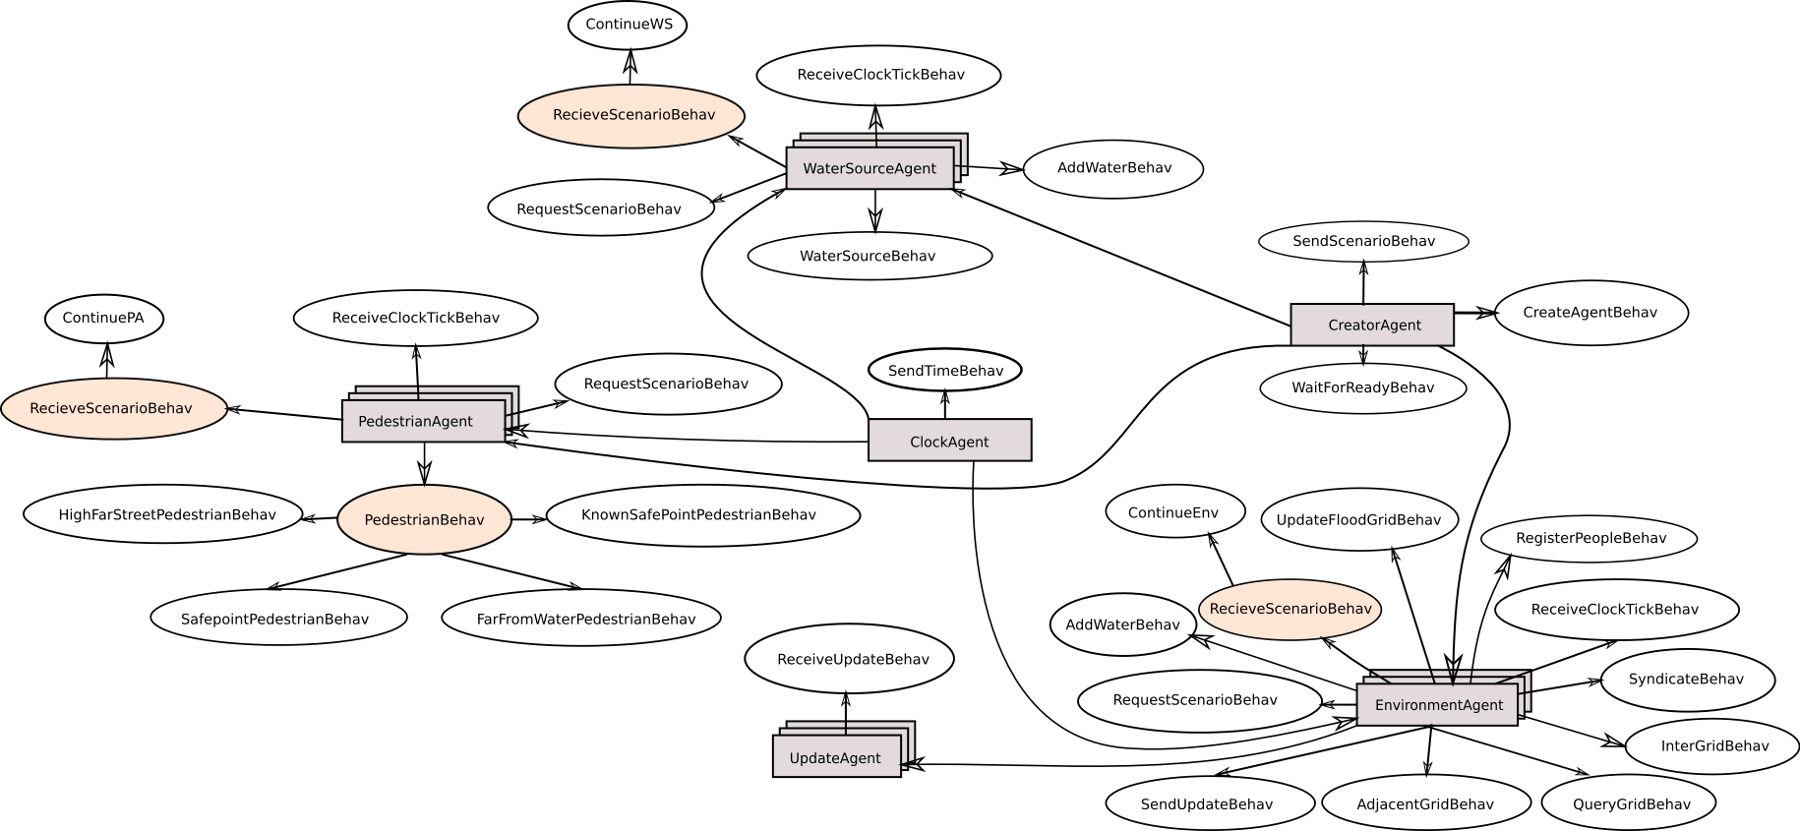
\includegraphics[height=100mm,angle=90]{figuras/cap5/agents.png}
 \caption{Esquema con todos los agentes}
\end{figure}

En programación con agentes lo habitual es que los agentes en sí no contengan
la lógica de su actividad, si no que tan sólo contienen el código de
inicialización y de finalización. Toda actividad que desarrolle el agente
durante su vida debe estar contenida en sus comportamientos, luego para que el
agente haga cualquier acción ha de añadírsele el comportamiento adecuado.

Para la programación de agentes utilizamos JADE, y JADE funciona mediante
herencia. Por ejemplo, para programar un agente hemos de extender la clase {\em
jade.core.Agent}. Y lo mismo para los comportamientos de los agentes, se
extiende la clase {\em jade.core.behaviours.Behaviour}. Una vez extendida la
clase correspondiente se implementan los métodos abstractos y se sobreescriben
los que se consideren necesarios.

Por ejemplo, en el caso de un agente, JADE proporciona una manera de
inicializarlo, que es sobreescribir el método {\em setup()}. JADE nos garantiza
que dicho método se ejecutará una única vez al crear el agente.

De la misma manera se trabaja con los comportamientos. Además JADE proporciona
múltiples clases de las que extender, estos comportamientos refinados -heredan
todos de {\em jade.core.behaviours.Behaviour}- facilitan la programación. Por
ejemplo, para un comportamiento que cree a otro agente lo habitual es sólo se
ejecute una vez, para ello se hereda directamente de {\em
jade.core.behaviours.OneShotBehaviour} y JADE nos asegura de que sólo se
ejecutará una vez.

A continuación pasamos a explicar los agentes del simulador. Por cada agente
hay un esquema de los comportamientos que utiliza, y en algunos de ellos -los
que inicien un diálogo con otros agentes- también hay un esquema de las
comunicaciones que mantienen.

Dichos esquemas de comunicación siguen el siguiente formato: A cada lado se
sitúa un agente, a la izquierda el que comienza el diálogo. Entre los agentes
hay flechas que representan mensajes, el sentido de la fecha denota al emisor y
al receptor. Sobre cada flecha va descrito, y en este orden, desde qué
comportamiento se envía, que comportamiento lo recibe, y de qué trata el
mensaje -tipo o contenido del mismo-. Obviamente el comportamiento que envía el
mensaje es del agente emisor, y el que recibe es del agente receptor.

\subsection*{Agente Creador}

La misión de este agente es la de crear al resto de agentes y lanzar la
simulación.

\begin{figure}[H]
 \centering
 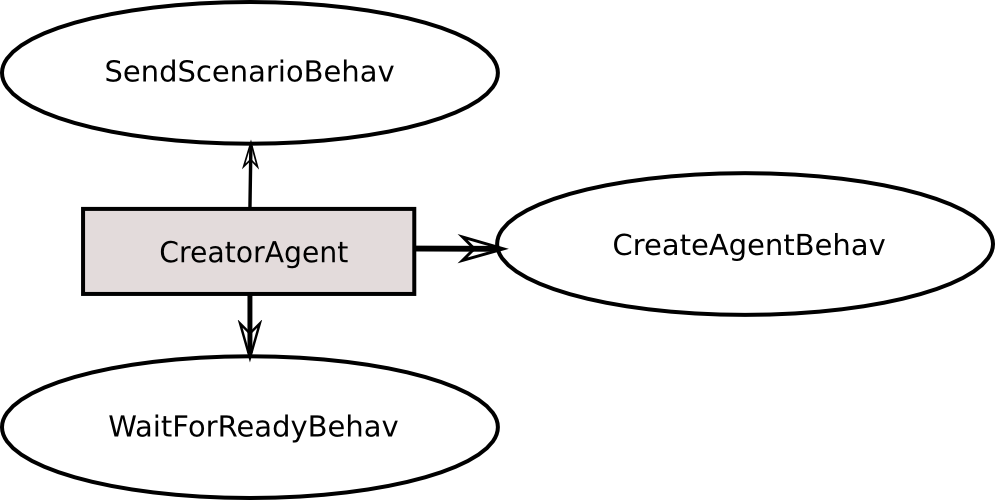
\includegraphics[width=100mm]{figuras/cap5/ag_creator.png}
 \caption{Agente Creador}
\end{figure}

Su ejecución consta de tres fases. En la primera procesa el fichero escenario y
crea a los agentes {\em Entorno}, a través del comportamiento {\em
CreateAgentBehav}, que es el comportamiento utilizado para crear agentes y que
se encuentra en el paquete {\em behaviours}. El agente se queda esperando a que
los agentes {\bf Entorno} terminen de inicializarse, para ello utiliza el
comportamiento {\em WaitForReadyBehav}, del mismo paquete.

Una vez listos, el agente {\bf Creador} pasa a la segunda fase en donde crea al
resto de agentes: {\bf Entradas de Agua}, {\bf Peatones}, etc, todo según se
describa en el escenario. Es necesario esperar a que se inicialicen los
entornos, dado que es un proceso lento (han de obtener las alturas y las
calles) y el resto de agentes los necesitan preparados pues les preguntan cosas.
Por último crea al agente {\bf Reloj} dando comienzo así a la simulación.

En la tercera y última fase, el {\bf Creador} se queda inactivo a la espera de
mensajes que soliciten el objeto escenario, enviándoselo a los agentes que
manden dichos mensajes. Esta actividad la realiza a través del comportamiento
{\em SendScenarioBehav}.

Este último comportamiento actúa como servidor del objeto escenario, y se
implementa mediante un {\em CyclicBehaviour} de JADE.

\subsection*{Agente Reloj}

Este agente apareció en nuestro sistema considerablemente tarde, por lo que
tuvimos que hacer bastantes cambios para incluirlo. Nació de la necesidad de
sincronizar los diferentes agentes de la simulación.

Esta necesidad quedó patente cuando generábamos ficheros KML con datos de
múltiples entornos. Al visualizar estos ficheros veíamos cómo zonas de la
simulación se adelantaban a otras, efecto que no se apreciaba fuera del KML
porque era consecuencia del desajuste de la fecha y hora de los entornos, no
porque no se hubiesen simulado al mismo tiempo.

En un primer momento implementamos un sistema que escogía arbitrariamente a un
agente {\bf Entorno} y lo designaba como reloj, el encargado de esta selección
era el agente {\bf Creador} -porque se trata del único agente del que no hay
puede haber múltiples copias en una simulación-. Los agentes {\bf Entorno} se
proponían como relojes cuando recibían agua de una {\bf Entrada de Agua}, pues
usaban éstas como forma de medir el tiempo. El {\bf Creador} escogía al primero
de ellos y éste se encarga de avisar al resto cada vez que se actualizaba el
reloj. Este sistema se demostró muy poco eficaz y provocó la aparición de los
mencionados desajustes.

La solución fue la creación del agente {\bf Reloj} y el establecimiento de un
tick de simulación. Los agentes sometidos a ese tick son todos aquellos cuya
tarea depende del tiempo simulado, que son los {\bf Entornos}, {\bf Entradas
de Agua} y {\bf Peatones}.

\begin{figure}[H]
 \centering
 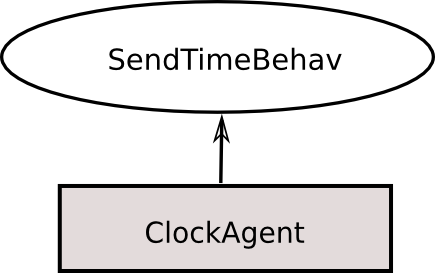
\includegraphics[width=50mm]{figuras/cap5/ag_clock.png}
 \caption{Agente Reloj}
\end{figure}

Este agente tiene un comportamiento de tipo {\em
jade.core.behaviours.TickerBehaviour}, que se ejecuta periódicamente según un
intervalo definido en el escenario. Cada vez que se ejecuta manda un mensaje a
los agentes comentados anteriormente, dando lugar a un nuevo paso de la
simulación. En dicho mensaje manda la fecha y hora dentro de la simulación,
correspondiente a ese paso. Todos los agentes que reciben estos mensajes lo
hacen a través del comportamiento {\em behaviours.ReceiveClockTickBehav}.

De esta forma se solucionan los problemas de sincronización entre agentes, se
eliminan los desajustes del KML, se soluciona el problema del cálculo de la
velocidad de los peatones e, incluso, se mejora la escalabilidad del sistema,
dado que aumentando el periodo permitimos que el simulador corra en máquinas
menos potentes.

Esta técnica de sincronización se utiliza mucho cuando se trabaja con JADE y
hay que sincronizar los agentes, pues JADE es de naturaleza asíncrona.

\begin{figure}[H]
 \centering
 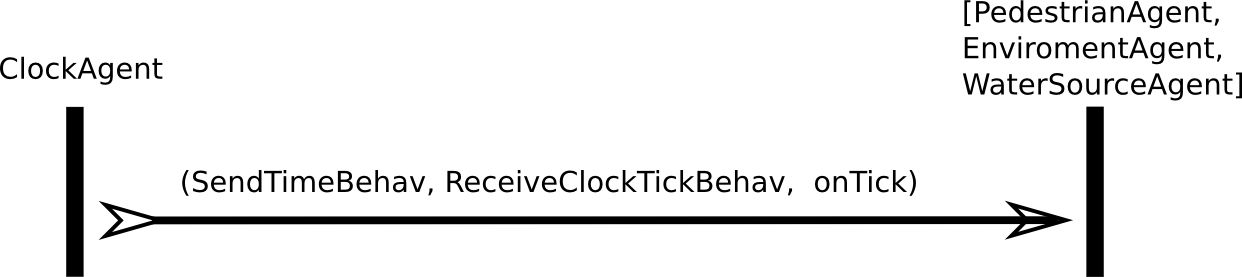
\includegraphics[width=120mm]{figuras/cap5/com_clock.png}
 \caption{Comunicaciones del agente Reloj}
\end{figure}

\subsection*{Agentes Entorno}

Los agentes {\em Entorno} son sin duda los más complejos y los más importantes
de cuantos forman la simulación. Su papel es manejar y mantener la información
del terreno simulado. Se encarga de obtener los datos de altura y calles, de
mover el agua de la inundación, de responder a los {\bf Peatones}, de enviar el
estado de la simulación a los agentes {\bf Actualización}, etc.

Durante su inicialización este agente obtiene los datos necesarios del terreno
que le toca simular, o de una base de datos o bien de un servicio web. La manera
en la que se descargan estos datos será explicada en la sección correspondiente.

Una vez inicializado el terreno, el agente crea y añade sus comportamientos, y
se registra en el servicio de ``páginas amarillas'' de JADE -{\em Directory
Facilitator} (DF)- para que el resto de agentes pueda encontrarlo. Por último
avisa al agente {\bf Creador} de que está listo para comenzar la simulación.

Para representar este terreno optamos por una maya hexagonal, que manejamos
mediante la clase {\em util.HexagonalGrid}. Cada agente {\bf Entorno} posee una
instancia de dicha clase con los datos de su trozo de simulación. Como es el
entorno el que posee los datos del terreno, proporciona también servicios de
consulta de dicha información al resto de agentes. Dichos servicios se
implementan mediante comportamientos del tipo {\em
jade.core.behaviours.CyclicBehaviour}, en particular se trata de los
comportamientos {\em behaviours.AdjacentsGridBehav} y {\em
behaviours.QueryGridBehav}.

\begin{figure}[H]
 \centering
 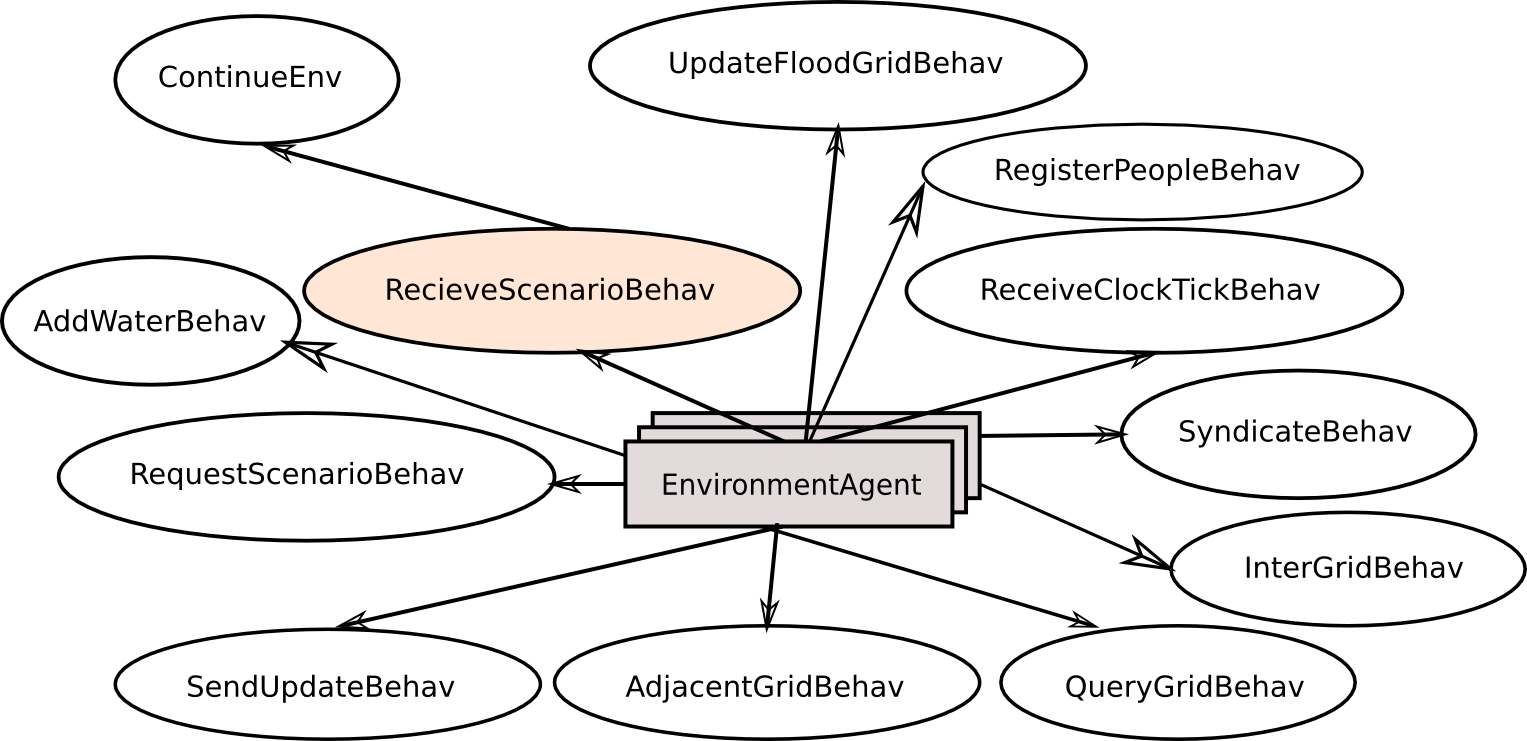
\includegraphics[width=130mm]{figuras/cap5/ag_environment.png}
 \caption{Agente Entorno}
\end{figure}

Los comportamientos {\em behaviours.flood.AddWaterBehav}, de tipo cíclico, y el
{\em behaviours.flood.UpdateFloodGridBehav}, de tipo periódico, son propios de
inundaciones. El primero recibe y procesa los mensajes de las entradas de agua,
añadiendo más agua a la simulación si fuera necesario -si resulta que la fuente
de agua no está a un nivel superior que el agua que la rodea, el nuevo agua se
desestima-. El segundo es el encargado de mover el agua por el terreno.

{\em behaviours.InterGridBehav} es un comportamiento que se encarga de la
comunicación entre {\bf Entornos}. Cuando, por ejemplo, el agua llega al borde
del terreno simulado por el agente, busca al {\bf Entorno} que simula el trozo
correspondiente y le avisa de que le llega agua, si es que existe tal {\bf
Entorno}.

El comportamiento {\em behaviours.SyndicateBehav} es el comportamiento
utilizado por los agentes {\bf Actualización} para darse de alta o baja en la
recepción del estado de la simulación.

{\em behaviours.people.RegisterPeopleBehav} es el comportamiento con el que se
comunican los {\bf Peatones} para avisar al entorno de su posición y salud.

\begin{figure}[H]
 \centering
 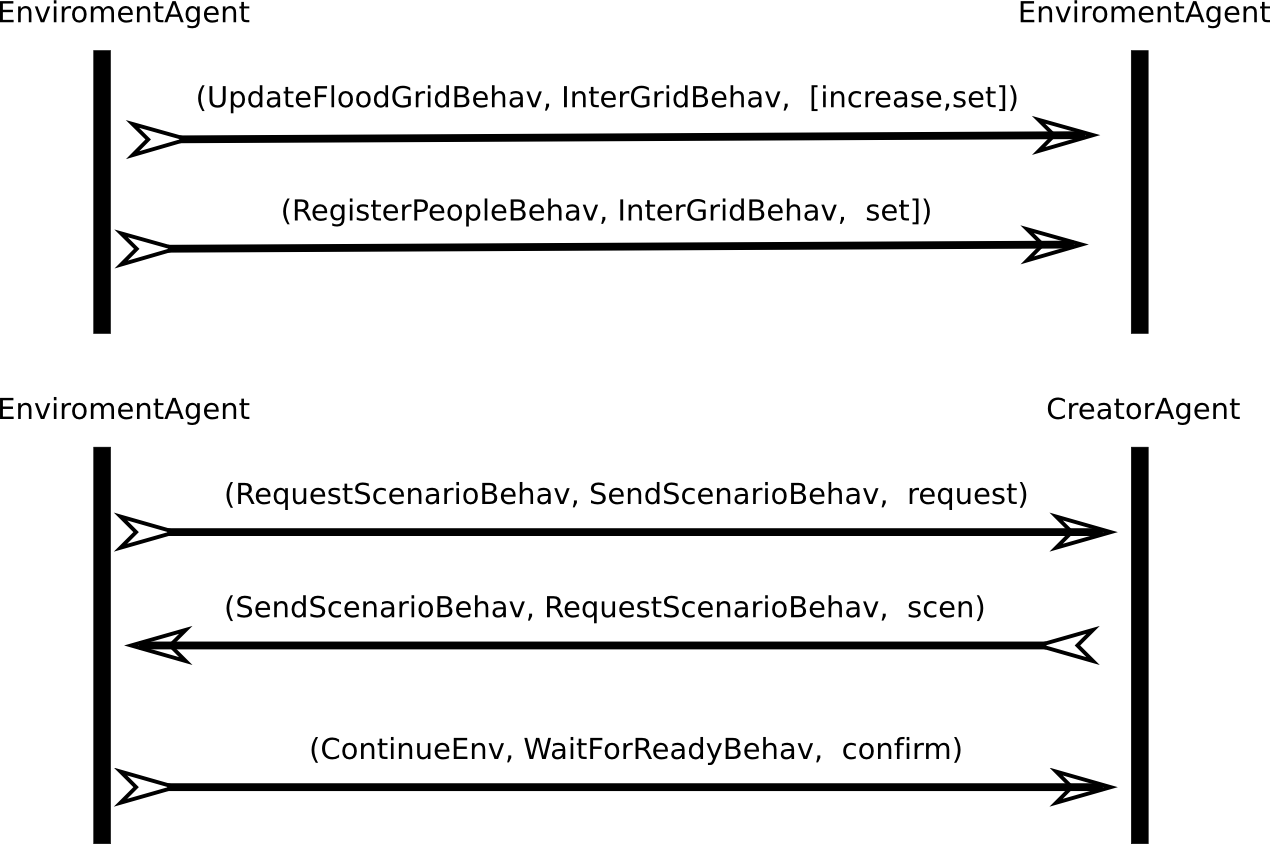
\includegraphics[width=120mm]{figuras/cap5/com_environment.png}
 \caption{Comunicaciones del agente Entorno}
\end{figure}

\subsubsection*{Casillas Adyacentes y Múltiples Entornos}

El {\bf Entorno} recibe muchas peticiones, normalmente de los {\bf Peatones},
solicitando las casillas adyacentes a una dada. El agente consulta su maya
hexagonal y devuelve las casillas pedidas.

El único problema es que un {\bf Entorno} sólo conoce lo que ocurre en el
terreno que simula, pero no los datos del resto de {\bf Entornos}. Para los
{\bf Peatones} esto es un problema, pues para ellos el que se simule con
múltiples {\bf Entornos} debería ser transparente. Esto significa que las
fronteras que separan los trozos de terreno de los diferentes agentes {\bf
Entorno} suponen una barrera a la visión de los {\bf Peatones}, lo cual no
tiene ningún sentido.

Para solucionar dicho problema tuvimos que refinar el comportamiento {\em
AdjacentsGridBehav}, y hacer que cuando detectase que la casilla de la que se
solicitan los adyacentes está más cerca del borde del terreno que la distancia
de visión pedida, entonces solicitase los adyacentes restantes a los agentes
{\bf Entorno} correspondientes.

Es decir, que cuando un agente {\bf Peatón} solicita los hexágonos adyacentes a
uno dado a un {\bf Entorno} concreto, puede estar involucrando a más agentes en
el proceso pero sin saberlo. Para los {\bf Peatones} este proceso es del todo
transparente.

\subsubsection{Movimiento del Agua}\label{waterMovement}

Dadas las limitaciones vistas en el \hyperref[cap2]{capítulo 2}, y sobre todo
dada nuestra intención de crear un modelo sencillo y abarcable, hemos
implementado un relativamente sencillo comportamiento para simular el
movimiento del agua. Dicho comportamiento es {\em UpdateFloodGridBehav}.

El funcionamiento del algoritmo es el siguiente:

\begin{enumerate}
 \item Se solicitan a la maya hexagonal las casillas cuyo nivel de agua ha sido
 modificado desde la última vez que se ejecutó el algoritmo.
 \item Se recorren dichas casillas, y se consulta el valor del agua y terreno
 de las casillas inmediatamente adyacentes.
 \item Si se encuentran casillas adyacentes más bajas entonces se mueve agua a
 dichas casillas -se mueve la mitad de la diferencia en altura, es decir, se
 iguala el nivel-. Si se encuentran casillas más altas se trae agua de dichas
 casillas.
 \item Todas las casillas cuyo nivel de agua haya sido afectado se marcan como
 modificadas, y serán revisadas por la siguiente pasada del algoritmo.
\end{enumerate}

Para el funcionamiento de este algoritmo cuando se simula en múltiples {\bf
Entornos} se hizo necesario incluir un borde exterior extra o corona a las mayas
hexagonales. Esta corona es del ancho de una casilla y mantiene el valor del
terreno y nivel de agua, aunque no se muestra en los visores. La utilidad de
esta corona es saber cuándo se debe pasar agua, y cuánta, a otros {\bf
Entornos}.

Cuando un {\bf Entorno} decide mover agua de una de sus casillas a una de la
corona comprueba a qué {\bf Entorno} pertenece dicha casilla. Si lo encuentra
le avisa de que ha añadido agua a la casilla. Si no lo encuentra es que es una
casilla fuera de la simulación con lo que el agua se pierde. El simulador
desconoce qué le ocurre a todo el agua que se sale de la simulación, por lo que
los bordes exteriores, no las fronteras entre {\bf Entornos}, son sumideros por
los que desaparece agua de la simulación. La cantidad de agua que desaparece
viene determinada por la altura del terreno, otra utilidad de la corona.

También ocurre que cuando un {\bf Entorno} modifica el nivel de agua de una
casilla del borde inmediatamente interior a la corona -es decir, el borde
exterior de su área de simulación- debe avisar del nuevo nivel al agente que
tenga esa casilla como corona, si es que lo hay.

Para manejar toda esta comunicación entre {\bf Entornos} creamos el
comportamiento {\em InterGridBehav}.

Como anécdota cabe comentar que en una primerísima versión del simulador,
cuando estábamos aún diseñándolo y haciendo pruebas, optamos por agentificar el
agua. De esta forma cada ``gota'' de agua era un agente que recorría el terreno
y escogía donde quedarse, inundando la casilla. El sistema funcionaba pero muy
poco escalable, dado que la cantidad de agentes agua era abrumadora. Lo
desechamos rápidamente y comenzamos el diseño del sistema actual.

\subsection*{Agentes Entrada de Agua}

Este tipo de agente es de lo más sencillo. Son agentes para nada inteligentes,
cuya única misión es enviar un mensaje al {\bf Entorno} correspondiente en cada
paso de la simulación avisándole de la cantidad de agua que debe añadir.

\begin{figure}[H]
 \centering
 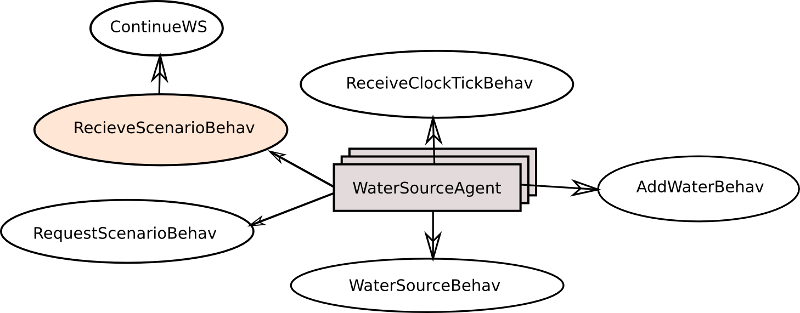
\includegraphics[width=120mm]{figuras/cap5/ag_water_source.png}
 \caption{Agente Entrada de Agua}
\end{figure}

En su inicialización el agente busca su {\bf Entorno}, para ello necesita
conocer el escenario de simulación que solicita al agente {\bf Creador}.
Consultando las coordenadas geográficas donde está situado y el escenario
descubre en qué trozo del terreno ha caído. A partir de ahí se limita a mandar
un mensaje en cada tick del {\bf Reloj}.

\begin{figure}[H]
 \centering
 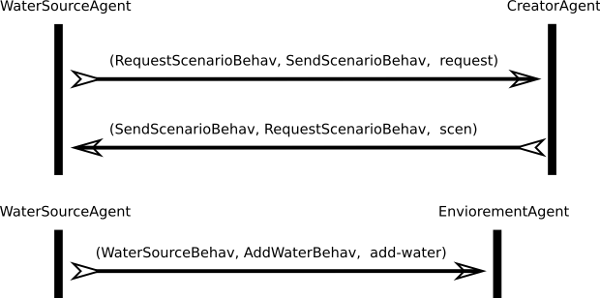
\includegraphics[width=120mm]{figuras/cap5/com_water_source.png}
 \caption{Comunicaciones del agente Entrada de Agua}
\end{figure}

\subsection*{Agentes Peatón}

Durante la inicialización estos agentes averiguan cuál es el {\bf Entorno} cuyo
terreno contiene su coordenada inicial, para ello utilizan el escenario que
solicitan al agente {\bf Creador}. Una vez inicializados comienzan a moverse
por el terreno tratando de salvarse de la inundación.

\begin{figure}[H]
 \centering
 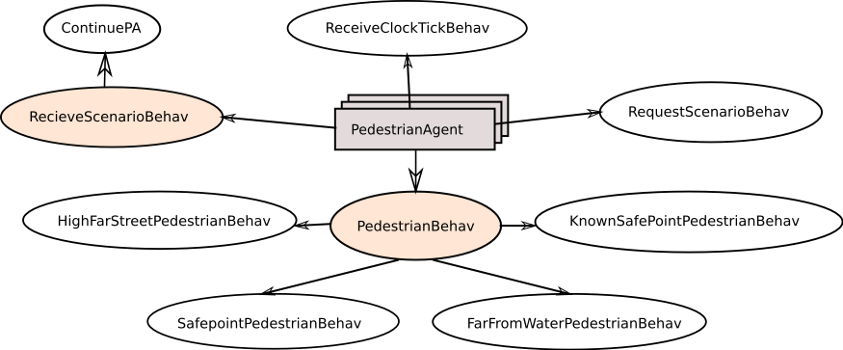
\includegraphics[width=135mm]{figuras/cap5/ag_pedestrian.png}
 \caption{Agente Peatón}
\end{figure}

Como hemos visto en el escenario de simulación, los agentes {\bf Peatón}
reciben una serie de parámetros de entrada. A saber:

\begin{description}
 \item[Posición inicial] Dado en coordenadas geográficas latitud,longitud.
 \item[Distancia de visión] Medida en hexágonos, representa cuantos hexágonos
 es capaz de ver el peatón en línea recta. Se utiliza a la hora de solicitar
 casillas adyacentes a la posición en ese momento.
 \item[Velocidad] La cantidad de hexágonos que la persona es capaz de recorrer
 en un único paso de simulación.
 \item[Objetivos] Coordenadas geográficas de los refugios que el {\bf Peatón}
 conozca desde el principio. Pueden ser más de uno, uno, o directamente ninguno.
\end{description}

El comportamiento base de todos los {\bf Peatones} funciona de la siguiente
manera:

\begin{enumerate}
 \item Solicitar casillas adyacentes según distancia de visión al {\bf Entorno}.
 \item Recibir casillas y escoger a cuál moverse.
 \item Si se ha escogido casilla, avisar al {\bf Entorno} de la nueva posición.
 Si no, volver al paso 1 sin moverse de la posición.
\end{enumerate}

Es en el segundo paso donde reside toda la complejidad, justo a la hora de
escoger a qué casilla moverse. Para facilitar la implementación de diferentes
comportamientos hemos implementado un comportamiento base abstracto, {\em
behaviours.people.PedestrianBehav}, del que heredar. Heredando de dicho
comportamiento lo único que hay que hacer es implementar un método {\em
choose(Set$<$Point$>$ adjacents)} que es dónde se escoge la casilla a la que
moverse.

Nosotros hemos ido perfeccionando y refinando el comportamiento de las
personas, habiendo desarrollado los siguientes -todos ellos en el paquete {\em
behaviours.people.flood}-:

\begin{description}
 \item[FarFromWaterPedestrianBehav] El primer y más simple de los
 comportamientos, el agente tan sólo escoge la casilla más alejada del agua
 que alcanzaba a ver.
 \item[HighFarStreetPedestrianBehav] Esta segunda aproximación es un poco más
 sofisticada pues tiene en cuenta también la altura de las casillas. Se pondera
 y se asigna una puntuación a cada casilla según lo alejada del agua que esté,
 y lo alta que sea. Escoge la casilla con mejor puntuación.
 \item[SafepointPedestrianBehav] Este comportamiento ya es bastante más
 complejo. Los agentes se desplazan según una dirección aleatoria, pero
 manteniéndola. De esta forma van recorriendo las calles de la ciudad, y
 cuando llegan a cruces de calles existe la posibilidad de que cambien de
 dirección y comiencen a recorrer alguna bocacalle. Cuando ven agua escogen la
 dirección contraria y huyen de ella, y cuando ven un refugio corren a él y se
 ponen a salvo.
 \item[KnownSafepointPedestrianBehav] La última evolución del comportamiento
 implica el conocimiento a priori por parte de los agentes de la posición de
 algún refugio. El agente trata de alcanzar algunos de los refugios que conoce,
 aunque si por el camino encuentra algún refugio se recoge en él. En caso de no
 tener objetivos o ser estos inaccesibles -la inundación le ha cortado el paso,
 por ejemplo- se comporta como el {\em SafepointPedestrianBehav}.
\end{description}

En este último comportamiento, el {\em KnownSafepointPedestrianBehav}, fue
necesario dotar al agente de memoria. Un problema que encontramos cuando
probábamos el comportamiento es que en ocasiones el agente se quedaba atascado
intentando atravesar edificios. Y es que la casilla más cercana al refugio
podía coincidir con su posición actual, dado que el cálculo de la distancia no
tiene en cuenta los edificios ni las calles. Al dotar de memoria al agente, y
penalizar severamente el moverse a casillas por las que acaba de pasar,
solucionó el problema. El agente prefiere dar un rodeo y alejarse temporalmente
del refugio a volver sobre sus pasos o quedarse quieto.

\begin{figure}[H]
 \centering
 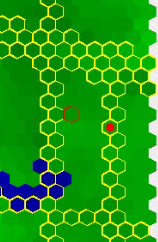
\includegraphics[width=35mm]{figuras/cap5/atasco.png}
 \caption{Peatón atascado}
\end{figure}

Como se puede apreciar en la imagen la casilla en la que se encuentra el peatón
-el punto rojo- es la más cercana al refugio -hexágono de borde rojo-. Esto
provocaba que el agente se quedase quieto u oscilase alrededor de dicha casilla.

Cabe destacar que no se han tenido en cuenta ni la capacidad de las calles ni
de los refugios, el número de personas que puede haber en una casilla es
ilimitado.

\begin{figure}[H]
 \centering
 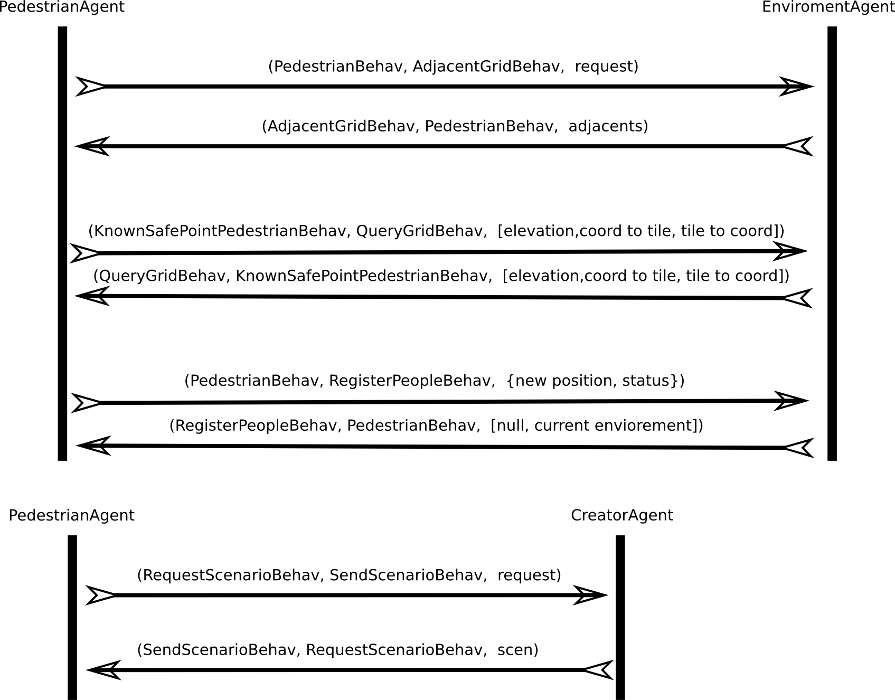
\includegraphics[width=135mm]{figuras/cap5/com_pedestrian.png}
 \caption{Comunicaciones del agente Peatón}
\end{figure}

\subsection*{Agentes Actualización}

Estos agentes nos permiten sacar información de la simulación. Durante su
inicialización lo que hacen es subscribirse a los agentes {\bf Entorno} que se
le pasen por parámetros.

Los {\bf Entornos} le enviarán periódicamente un objeto de tipo {\em
util.Snapshot} con el estado de la simulación en ese momento.

\begin{figure}[H]
 \centering
 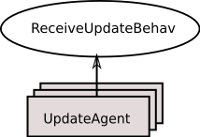
\includegraphics[width=50mm]{figuras/cap5/ag_update.png}
 \caption{Agente Actualización}
\end{figure}

Todos los agentes {\bf Actualización} tiene un objeto cliente, que debe
implementar la interfaz {\em util.Updatable}. Son estos objetos los que
procesan los {\em snapshots} y producen algún resultado.

Por ejemplo, los generadores KML o los extractores de estadísticas, interactúan
con la simulación a través de un agente {\bf Actualización}, y ambos
implementan {\em Updatable}. Se pueden escribir nuevos clientes para estos
agentes sin tener que modificarlos, dado que reciben por parámetros el nombre
de la clase del cliente de la que crean la instancia mediante reflexión.

\begin{figure}[H]
 \centering
 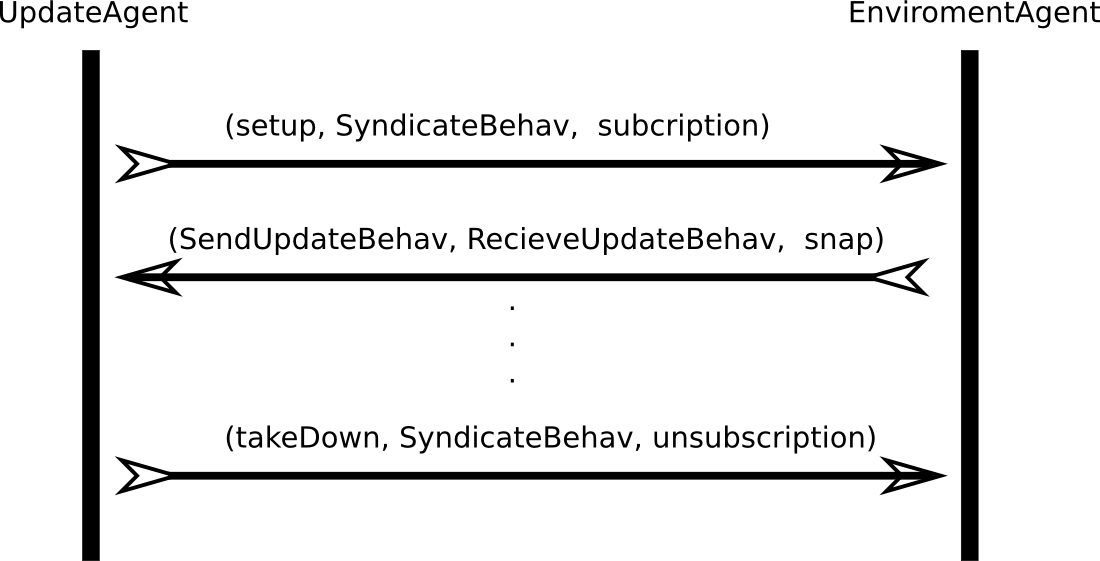
\includegraphics[width=100mm]{figuras/cap5/com_update.png}
 \caption{Comunicaciones del agente Actualización}
\end{figure}

\section*{Maya Hexagonal}

Sobre la rejilla es donde se van a realizar todos los cálculos de la simulación,
por lo tanto dispone de todos los métodos para manipular y obtener la
información contenida en ella. También contiene funcionalidad básica como
obtener todos los adyacentes a un punto, o calcular la distancia que separa a
dos casillas. La implementación de la maya hexagonal se encuentra en la clase
{\em util.HexagonalGrid}.

La manera de almacenar la información es a través de matrices cuadradas, los
métodos de acceso y cálculo de adyacentes la hacen parecer una maya hexagonal a
quien los usa. Todas las matrices almacenan datos de tipo {\em short}, pues no
es necesario un rango mayor y así se ahorra memoria. Todas las matrices son de
la misma dimensión.

\subsection*{Matriz de Alturas}

El rango del tipo básico {\em short} en Java va desde -32768 hasta 32767, y
dependiendo de la precisión en altura que se esté utilizando el rango en metros
será menor o mayor que éste.

\subsection*{Matriz de Agua}

Para el caso de inundación se añade esta matriz, que a diferencia de la matriz
de alturas, sólo almacena valores positivos -no tiene sentido un nivel de agua
negativo-. Los valores de esta matriz cambiarán a lo largo de la simulación,
otra diferencia con respecto a la matriz de alturas.

Sumando los valores de una casilla en las matrices de alturas y agua se obtiene
la altura total del terreno en ese punto.

\subsection*{Matriz de Calles}

Esta matriz no se modifica una vez rellena, y almacena valores clave que definen
el tipo de casilla del que se trata. Valores del tipo ``calle'', ``avenida'',
``autovía'', ``hotel'', ``río'', etc.

Gracias a estos valores los agentes tienen una representación de las
construcciones y calles que los rodean.

\subsubsection*{Tipos de Calles}

Para saber en qué tipo de calle nos encontramos nos ayudamos de la información
de OSM, que viene categorizada en grupos, tales como ``carreteras``, ''puntos
de interés``, ``vías de agua``, etc. A cada grupo le asignamos un rango de
valores, teniendo en cuenta el número de subgrupos que tiene. Por ejemplo, el
grupo ''carreteras`` tiene múltiples subgrupos, como pueden ser ''calle``,
''avenida``, ''autovía``, etc.

Estos valores los identificamos por medio de constantes globales; y se
comparan mediante funciones estáticas, que nos devuelven el tipo concreto o los
valores padre -para los subgrupos-.

\subsubsection*{Prioridad de la Información}

Ocurre que en ocasiones varios elementos caen en la misma casilla, pues están
muy cercanos geográficamente y les corresponde el mismo hexágono. Pero en cada
casilla sólo podemos almacenar un valor, por lo que rellenamos la matriz de
forma que se sobreescribe el valor que hubiera si el nuevo valor es mayor que el
viejo. Así nos aseguramos que la información que consideramos más prioritaria
-de mayor valor- permanezca en la matriz.

\subsubsection*{Intersecciones}

A veces es útil, sobre todo en el caso de las calles, saber cuando se cruzan
dos o más elementos. Para ello, a la hora de sobreescribir valores, si nos
encontramos con que había un valor igual al que nosotros queremos insertar,
incrementamos en una unidad el valor que hubiese -haciéndolo impar-.

Obviamente para que este sistema funcione, los valores que insertemos
normalmente en la matriz -cuando no se sobreescribe ningún valor- tienen que ser
todos pares. Así si el valor de una casilla es impar sabemos que en ese punto
hay una intersección de dos elementos.

\subsection*{Coronas}

Como se comentó en la sección del \hyperref[waterMovement]{movimiento del agua}
de los agentes {\bf Entorno}, las mayas hexagonales disponen de una corona, o
borde extra, de casillas. Esta corona -de ancho un único hexágono- contiene los
datos de altura y nivel de agua de casillas que pueden pertenecer a {\bf
Entornos} vecinos.

La necesidad de establecer estas coronas viene de poder efectuar las
simulaciones en más de un {\bf Entorno}, pues teníamos que crear un sistema para
actualizar valores de casillas en los {\bf Entornos} vecinos.

De esta forma, cuando se modifica la información de una corona, el agente {\bf
Entorno} busca qué otro agente {\bf Entorno} -si que lo hay- posee dicha
casilla y le avisa de la actualización realizada. Así se mantiene la coherencia
entre {\bf Entornos} y el paso de uno a otro se vuelve transparente para el
resto de agentes.

\subsection*{Coordenada a Casilla, y Viceversa} \label{coordToCasilla}

El paso de coordenada geográfica a coordenada en la maya, y viceversa, es un
problema complejo que ha requerido un considerable esfuerzo. Hay que tener en
cuenta que la maya es hexagonal, y que la tierra no es plana.

\subsubsection*{Incrementos} \label{incrementos}

Para poder convertir la posición de una casilla a una determinada coordenada
geográfica hemos optado por la técnica de los incrementos, en vez de complicados
cálculos trigonométricos terrestres.

La técnica consiste en hallar la diferencia en grados decimales entre los
extremos del mapa, y dividirla entre el número de filas y columnas. Con esto
obtenemos el incremento en latitud o longitud que hay entre cada casilla de
nuestra rejilla.

Debido a la forma de la rejilla hexagonal tenemos que tener en cuenta que las
filas impares tienen un offset de \begin{math}^1/_2\end{math} de incremento de
latitud, y que las columnas tienen un incremento de \begin{math}^3/_4\end{math}
de incremento de la longitud.

De esta forma tan sencilla podemos hacer las conversiones de ''casilla a
coordenada``.

\subsubsection*{Discretización}

El problema de ''coordenada a casilla'' es un poco más complejo, puesto que al
trabajar con una coordenada tenemos que aproximar a una casilla en concreto
-la coordenada, muy probablemente, no va a coincidir con el centro de ningún
hexágono-.

Para ello primero realizamos una aproximación a grandes rasgos intentando
averiguar la casilla, sin embargo la forma de las casillas es hexagonal, por lo
que hay que asegurarse de que la casilla sea la correcta. Se refina la casilla
escogida calculando la distancia al centro de los hexágonos, escogiendo siempre
la más cercana. Pero como las casillas son hexagonales, no circulares, siempre
existe una posibilidad de error.

De esta forma perdemos un poco de información, pero los errores cometidos por
este sistema no superan el \begin{math}0.7\%\end{math}.

\section*{Especialización: Múltiples Desastres}

Siguiendo el estilo de JADE, con el que se trabaja a través de los mecanismos
de herencia de Java, hemos diseñado nuestro simulador para que se pueda
extender a múltiples desastres mediante herencia.

Por ejemplo, clases como {\em Scenario} o {\em HexagonalGrid} no se pueden
instanciar directamente, si no que hay que utilizar las clases hijas {\em
FloodScenario} y {\em FloodHexagonalGrid}. De la misma manera, implementando
nuevas clases hijas que sobreescriban de otra manera los métodos se podría dar
soporte a nuevos tipos de desastres naturales.

Las clases padres dan funcionalidad básica y común a todos los desastres. Por
ejemplo, {\em HexagonalGrid} mantiene las matrices de alturas y de calles,
mientras que es {\em FloodHexagonalGrid} la que añade la matriz de agua.

\section*{Elevación del Terreno}

Para la obtención de alturas utilizamos servicios de información en la red. Por
desgracia la obtención de estos datos puede resultar lenta, por lo que se hizo
necesario implementar una caché de alturas.

\subsection*{Caché de Alturas}

Obtener todas las alturas de todas las casillas cada vez que necesitemos
simular un escenario no es viable. La solución que nosotros implementamos es
almacenar en local los datos para utilizarlos de nuevo en posteriores
simulaciones, o incluso para poder reutilizarlos en otras máquinas.

El almacenamiento se realiza en un servidor de base de datos, al que se accede
a través de JDBC\footnote{Java Database Connectivity:
\url{http://java.sun.com/products/jdbc/overview.html}}. Por ahora están
soportados por el simulador los servidores MySQL, PostgreSQL y SQLite, pero
sería muy sencillo incluir más servidores siempre que haya un driver para JDBC.

La base de datos sólo contiene una tabla, de nombre Elevations, con tres campos:

\begin{center}
\begin{tabular}{ | l | c | r | }
\hline
{\bf Campo} & {\bf Tipo de datos} \\ \hline
Lat & DOUBLE \\ \hline
Long & DOUBLE \\ \hline
Elev & DOUBLE \\ \hline
\end{tabular}
\end{center}

El simulador intenta obtener los datos de la base de datos local, para ello
busca las alturas de las coordenadas que caigan dentro del hexágono y hace la
media de los resultados, y en caso de que no haya ninguna altura en la base de
datos la descarga del servicio web y la añade.

Es posible añadir nuevas fuentes de datos de alturas al simulador. Para ello es
necesario implementar el cliente del nuevo servicio cumpliendo con la interfaz
{\em elevation.ElevationService}.

\section*{Open Street Maps}

OSM permite la descarga de ficheros XML que contienen toda la información de
sobre las calles, puntos de interés, etc, contenidas en unas coordenadas
determinadas.

La {\em url} para descargar estos ficheros se compone de la siguiente manera: 
{\em dirección base + coordenada suroeste + coordenada noreste}. El fichero
descargado tendrá el mismo nombre que la petición.

\subsection*{Parsear XML}

La información viene codificada en un fichero XML siguiendo el estándar de OSM.
Para poder extraer la información es necesario parsear el fichero. Para ello
utilizamos JAXB\footnote{Java Architecture for XML Binding: 
\url{https://jaxb.dev.java.net/}}, que es una librería para recorrer ficheros
XML. 

Mientras realizamos el recorrido del fichero hay que identificar la información
de las etiquetas y almacenarla en nuestra estructura de datos para poder
utilizarla de una forma mas cómoda. El diseño de las clases que hemos
implementado para almacenar la información es muy parecido a la jerarquía de
información que sigue OSM.

La clase principal es {\em OsmMap}, que contiene toda la información que nos da
OSM. {\em OsmWay} es para la etiqueta {\em way} (camino o vía) de OSM, y {\em
OsmMember} para los caminos compuestos. {\em OsmRelation} para los ríos y
parques, y {\em OsmNode} para los puntos simples y puntos de interés. Para
almacenar la información extra creamos {\em OsmTag}.

\subsubsection*{Filtro de Información}

{\em OsmTag} contiene dos atributos principales, clave y valor. Nos valemos de
estos dos atributos para almacenar la información extra que nos ofrece OSM, como
el nombre de la calle, el tipo de calle, o si se trata de un edificio o un
parque. Con esta información podemos determinar con qué tipo de objeto estamos
tratando, y asignarle un valor concreto en la matriz de calles de cada {\bf
Entorno}.

También nos valemos de esta información para filtrar los datos. Hasta ahora
hemos optado por almacenar sólo con la información que queremos, desechando el
resto; pero si algún día se añade un nuevo tipo de información que no se
almacena, únicamente habría que añadirlo al filtrado de etiquetas.

\subsection*{Dibujar Calles}

OSM nos da la información de las calles como listas de coordenadas geográficas
que hay que unir con líneas rectas. Esto plantea dos problemas.

Uno de ellos, el manejo de las coordenadas geográficas, lo resolvemos pasando de
coordenadas a casillas, como ya hemos explicado en el apartado
\hyperref[coordToCasilla]{{\em Coordenada a Casilla, y Viceversa}}.

El otro problema es crear una línea recta a partir de dos puntos, teniendo en
cuenta que el plano es hexagonal, consiguiendo siempre que sea conexa.

Para hallar los puntos que componen las rectas nos valemos de la ecuación
matemática de la recta, y a partir de su pendiente podemos averiguar cual será
el próximo punto.

Para el problema del mapa hexagonal usamos dos técnicas. La primera es buscar el
siguiente punto de la recta avanzando la mitad de distancia de una casilla, así
hacemos los cambios gradualmente y nos aseguramos la conexión del camino con
las casillas. Pero así no solucionamos el problema que presentan las diagonales,
para esto usamos vectores de direcciones para corregir el rumbo y adaptarlo a la
malla hexagonal. Es vital que las calles sean conexas y no aparezcan cortadas
por un mal paso de coordenadas a casillas.

Al usar estas técnicas obtenemos más puntos de los necesarios para pintar la
recta, por lo que guardamos siempre la casilla anterior a la que se calcula en
ese momento y si es la misma, no la pintamos.

\subsection*{Rellenar Figuras}

Existen tres figuras diferentes a la hora de dibujar los mapas. Los puntos
simples, las líneas rectas y las polilíneas cerradas. Estas últimas se componen
de varias líneas rectas, que a su vez son una sucesión de puntos. Y en muchas
ocasiones estas figuras encierran espacios que son de un único tipo, y hay que
marcar todas las casillas contenidas en dicho espacio con el tipo correcto. Es
el caso de ríos, parques, etc.

\subsubsection*{Polilíneas Cerradas}

Es necesario hallar los puntos que encierra una línea, es un problema de
geometría computacional. Este problema aparece cuando queremos reflejar la
extensión de un río o de un parque, o cualquier otra superficie que ocupe más de
una casilla.

Es un problema muy conocido en geometría computacional por lo que hay muchos
algoritmos sencillos que lo resuelven; que dada una lista de puntos que
describen un polígono, te dicen si otro punto está dentro del polígono o no.

Una vez identificadas las líneas cerradas, que son aquellas en las que el primer
punto de la lista es igual al último punto, simplemente hay que aplicar el
algoritmo y rellenar las zonas con el valor adecuado.

\subsubsection*{Relaciones}

Sin embargo, existen otras figuras más complejas, como las orillas de los ríos
o las costas. OSM también nos da esta información, pero no es tan sencilla de
interpretar ya que sólo nos proporciona la línea de la orilla y a qué río
pertenece.

El problema es averiguar qué casillas rellenar y cuáles no, por ejemplo, en el
caso de encontrar la orilla de un río hay que averiguar en qué dirección está
el agua, y en cuál la tierra. Incluso puede complicarse más si dentro del área
de simulación sólo aparece una de las dos orillas del río. OSM ya prevé este
problema, y cuando pedimos la información de un lugar nos devuelve también
información de los alrededores. Si en nuestra zona sólo aparece una orilla del
río, OSM nos da la información también de la otra orilla. De esta forma, podemos
calcular el cauce del río aunque esté fuera de nuestro mapa, y pintar sólo
aquellas regiones que estén dentro del mismo.

Una vez más, la forma que tiene OSM de organizar los datos nos da la solución
a este problema. Porque simplemente encadenando las listas de puntos de las dos
orillas del río obtenemos la figura que envuelve al agua del río, con lo que
pasamos a tener el problema anterior, de fácil solución, que es rellenar una
polilínea cerrada. Para la costa, y otras formaciones de agua, o figuras
complejas, es equivalente.

\subsection*{Intersecciones de Caminos}

Además del tipo de camino, que es lo que estamos guardando en la matriz de
calles del {\bf Entorno}, podemos almacenar de una forma inteligente información
extra sobre las calles. Como por ejemplo el que una casilla en concreto forme
parte de una intersección entre calles, ahorrándole a los agentes la necesidad
de mirar las casillas adyacentes para detectarla.

La forma de almacenarlo es simplemente dar por defecto un valor par a todos los
tipos de caminos, y si alguna vez un camino se cruza con otro -siempre y cuando
sean del mismo tipo- se guarda en la casilla un valor impar -se incrementa en
una unidad el valor anterior-.

De esta manera tan simple podemos identificar y almacenar las intersecciones
entre calles.

\section*{Generador de KML}

El generador de ficheros KML, que se usa a través de un agente {\bf
Actualización} e implementa la interfaz {\em Updatable}, recibe el estado de la
simulación periódicamente y lo procesa. Este procesado no es trivial y presenta
algunos escollos que hemos tenido que superar.

El visor de KML puede recibir información de varios {\bf Entornos}, ya que al
utilizar todas las mayas índices absolutos la integración de éstas es directa.

KML permite asignar una fecha y hora a los polígonos que se van a dibujar, de
esta manera se puede crear una animación. A la hora de plasmar los resultados
de la simulación utilizamos esta capacidad para animarlos.

Creamos la clase {\em KmlPolygon} para tratar los polígonos en KML de manera
sencilla. Toda la información de la simulación la tenemos que representar por
medio de polígonos en el KML, con lo que facilitar la manipulación de estos era
vital. La clase nos facilita la creación y la asignación de las propiedades que
queremos que tenga nuestro polígono.

Para cada polígono contamos con la posición, la forma, la altura, el color, y la
transparencia. Haciendo un buen uso de estas características podemos mostrar
mucha información de una forma eficaz y elegante.

\subsection*{Bordes}

Nos enfrentamos a dos problemas: Las posiciones de los polígonos nos vienen
dadas a través de un única coordenada, pero nosotros para dibujar el polígono
necesitamos conocer los seis lados. Y el segundo problema es cómo reducir el
número de polígonos y lados a pintar en el KML, para que no se generen archivos
gigantescos imposibles de visualizar.

Hallar los seis vértices del polígono se resuelve fácilmente con los
\hyperref[incrementos]{incrementos en latitud y longitud} y un poco de
trigonometría.

El otro problema es mucho más complicado y no se resuelve fácilmente. La
simulación produce mucha información que reflejar en un solo archivo. Por
cada casilla inundada tenemos siete coordenadas, si eso lo multiplicamos por las
casillas inundadas y por el número de instantáneas, acabamos teniendo ficheros
de tamaño muy considerable. Si el fichero se vuelve demasiado pesado tendremos
problemas a la hora de abrirlo con un visor.

Para poder almacenar la mayor cantidad posible de datos usamos la versión KMZ
de los archivos -que no es más que versiones comprimidas en zip de los
archivos KML normales-, y además agrupamos las casillas inundadas al mismo
nivel en un único polígono.

Esto quiere decir que si tenemos un conjunto de casillas adyacentes con el
mismo nivel podemos agruparlas. Estas casillas pasan a dibujarse mediante un
único polígono, con lo que sólo tenemos que almacenar en el KML la forma de su
perímetro, no los hexágonos completos de todas las casillas que contiene.

Para implementarlo hacemos uso, otra vez, de conocimientos de geometría
computacional y del operador borde. Dicho operador nos permite hallar el
borde de cualquier figura.

% TODO poner fórmula matemática con un esquema o algo

% TODO explicar bien las listas de adyacencias, no con dos frases mal puestas

\subsection*{Color y Transparencia}

Como ya hemos comentado anteriormente, nos valemos del color para representar
la información de manera intuitiva. Azul para el agua, verde para personas a
salvo, etc.

KML permite asignarle color a las figuras a través de estilos, así que
simplemente creamos unos estilos y los asignamos a los polígonos. El color se
calcula para cada uno de los objetos, y es común para los objetos equivalentes.
Por ejemplo, en el caso del agua, si un polígono tiene la misma altura que
otros, todos tendrán el mismo color y transparencia por ser equivalentes.

Para las personas funciona igual, les asignamos colores (y una altura de 5
metros para que sean fácilmente identificables) y ninguna transparencia. Así
tenemos que las personas que están a salvo en refugios tendrán el color verde,
las personas que se encuentren en peligro corriendo por las calles tendrán el
color amarillo, y las personas que se hayan fallecido tendrán color gris.

Con este sencillo método podemos representar la información de manera muy
visual y expresiva.

\section*{Visor Bidimensional}
\subsection*{Múltiples escenarios}
\section*{Estadísticas}
Siguiendo la misma estrategia que los demás objetos que se actualizan
periódicamente, hemos diseñado un agente estadístico que se encarga de recoger
información de cada estado de la simulación.

Recogiendo la información deseada, en nuestro caso, el estado de las personas,
y el tiempo de la simulación, podemos hacer una evaluación estadística de la
evolución de la inundación, sabiendo cuales han sido las zonas donde mas
personas han perecido, o salvado y la hora en la que sucedió.
\subsection*{Múltiples Escenarios}
%Soporte para varios escenarios
Nuestra simulación puede tener mas de un escenario, por ello necesitamos
identificar de que escenario estamos recogiendo los datos, esto lo realizamos
simplemente añadiendo una columna con el identificador del escenario.
\subsection*{Ficheros CVS}
%Es lo mas comodo para las estadisticas
Los ficheros CSV\footnote{Valores Separados por Coma :
\url{http://es.wikipedia.org/wiki/CSV}} son muy fáciles de escribir y leer y la
forma mas simple de almacenar información. Por ello los hace ideales para
nuestro propósito de recoger una serie de estadísticas y guardarlas en un
fichero que sigue una forma estándar de almacenar los datos y que es reconocida
por la mayoría de hojas de cálculo y fácilmente se pueden generar gráficas a 
partir de estos ficheros.
%%% Local Variables:
%%% mode: latex
%%% TeX-master: "../dissim"
%%% End: